\chapter{Matrix Product States}
Attempts to perform numerical analysis of quantum many-body systems using exact diagonalisation are highly limited by system sizes. Due to the large number of possible configurations in a many-body scenario and entanglement coupling various degrees of freedom of the system, the Hilbert space grows too large for exact methods to search.
Consider the Bose-Hubbard model described in eq. \eqref{BHhamil}. The dimension of the corresponding Hilbert space is
\begin{equation}
	D_{\mathcal{H}} = \frac{(N+N_p -1)!}{N_p ! (N-1)!} \; ,
\end{equation}
where $N$ is the number of sites, and $N_p$ is the number of particles. For unit occupancy, $N_p / N = 1$, the Hilbert space grows exponentially with the system size \cite{Dong}. Therefore, descriptions using exact diagonalisation are only possible for small systems.
The invention of the density-matrix renormalization group
(DMRG) marked a turning point for numerical descriptions of quantum many-body systems, as it remains the most powerful method to study one-dimensional lattices \cite{White1992,White1993}. One of the defining differences between the DMRG method and exact diagonalisation is scaling of entanglement in the quantum states. In the DMRG description, systems automatically follow an area law, whereby only a tiny corner of the Hilbert space has to be considered when searching for ground states \cite{Cramer}.\\
Matrix Product States (MPS) are parametrizations of (typically) one dimensional states, where the states and operators are decomposed into networks of tensors. In this description of quantum states it is very easy to measure local properties of quantum many-body systems, and correlations can be computed very efficiently. The matrix product state description has surfaces several times under different names, most notable in \cite{Baxter1968}. However, the connection between the DMRG method and the MPS description made in \cite{Ostlund1995, Dukelsky1998} opened up the possibilities for performing time evolution, finite temperature analysis, and much more \cite{schollwock}.


\section{Entanglement in Quantum Systems and Area Laws}
Entanglement is a fundamental property of quantum mechanics responsible for correlating different degrees of freedom within a quantum system. Thus, the individual parts of a quantum system can not be described alone, as entanglement with the remainder of the system has to be taken into consideration. This drastically complicates any description of the system, which is why exact descriptions of many-body systems are almost impossible. CITE \\
The measure of entanglement within a quantum many-body system is the entanglement entropy, although it is often more instructive to look at the bipartite entanglement entropy, which measures the entanglement between two partitions of the system.
Consider a bipartition of the Hilbert space $\mathcal{H} = \mathcal{H}_A \otimes \mathcal{H}_B$. A state $\ket{\psi} \in \mathcal{H}$ can be decomposed using the \textit{Schmidt decomposition} as
\begin{equation}
	\ket{\psi} = \sum_{\alpha} \Lambda_{\alpha} \ket{\alpha}_A \otimes \ket{\alpha}_B \; ,
\end{equation}
where the states $\{ \ket{\alpha}_{A(B)} \}$ form an orthonormal basis of $\mathcal{H}_{A(B)}$, and $\Lambda_{\alpha} \ge 0$ are the Schmidt coefficients fulfilling $\sum_{\alpha} \Lambda_{\alpha}^2 = 1$ CITE. If only one term contributes to the Schmidt decomposition, the state is obviously a product state i.e. the two parts of the Hilbert space are not mutually entangled. More terms, on the other hand, implies that the state is entangled. From the Schmidt decomposition one can determine the reduced density matrix
\begin{equation}
	\rho_A = \Tr _B \ket{\psi}\bra{\psi} = \sum_{\alpha} \Lambda_{\alpha}^2 \ket{\alpha}_A \bra{\alpha}_A \; .  
\end{equation}
From this one can determine the entanglement entropy of the chosen bipartition, which is defined as the von-Neumann entropy, $S$, of the reduced density matrix given by CITE
\begin{equation}
	S = - \sum_{\alpha} \Lambda_{\alpha}^2 \log \Lambda_{\alpha}^2 \; .
\end{equation}
Quite often, one is not conserned with the actual entanglement entropy of the system, but rather how it scales when the region in question grows in size. It is natural to assume that the entanglement entropy scales with the systems size, the \textit{volume} of the system, since this is the case for thermal systems. However, ground states of quantum many-body systems often follow an \textit{area law}, meaning that the scaling of the entropy is linear in the boundary area of the region. This is especially the case for systems with a gapped and local Hamiltonian \cite{Cramer}.\\
In a one dimensional lattice the boundary of a bipartition consists of only one site. Hence, the entropy will be bounded by a constant independent of the size of both the system and the subsystem, if the system follows an area law. This can be understood intuitively, as only degrees of freedom within the correlation length, $\xi$, of the boundary will be entangled, no matter where in the system the boundary is present \cite{Hastings2007}.\\
This observation is the key to the success of numerical computations for one-dimensional systems, as one only has to consider a small region of the Hilbert space when performing a variational search for the ground state. A highly efficient way of describing one dimensional systems is through Matrix Product States (MPS), which follow an area law by default, as they are constructed through a series of Schmidt decompositions.


\section{Construction of an MPS} \label{sec:construct_MPS}
Matrix products states are parametrisations of one dimensional quantum states through a product of tensors. This parametrisation is especially intuitive for lattice systems, as each lattice site can be represented by a single tensor. These tensors have two different kinds of indices; \textit{physical indices}, $j$, which corresponds to the physical states at a given site, and \textit{bond indices}, which serves to connect neighbouring sites. Tensors can be merged by contracting the bond connecting them, which is achieved by summing over their common index. Hence, equations involving matrix product states tend to grow quite long, whereby they often are described through diagrams. In the diagrammatic representation the physical indices are marked by vertical legs, while bond indices are marked by horisontal legs. When two tensors are connected by a leg, it means that the corresponding bond is contracted. Further details and examples regarding tensor diagrams can be found in Appendix \ref{chap:diagrams}.\\

Consider a chain of $N$ sites with each site having a $d$-dimensional local Hilbert space $\{ \ket{j_n} \}$, where $n = 1, \ldots, N$. Thus, an arbitrary quantum state of this system reads
\begin{equation}
	\ket{\psi} = \sum_{j_1, \ldots, j_N} c_{j_1 \ldots j_N} \ket{j_1, \ldots, j_N} \; .
	\label{eq:arbstate}
\end{equation}
This description of a general state can be parametrised to the MPS form by applying successive Schmidt decomposition. However, in practice this is done through Singular Value Decompositions (SVD), as these are faster to perform numerically. The two approaches are equivalent, as the singular value decomposition is essentially a restatement of the Schmidt decomposition CITE.
Through an SVD, an arbitrary matrix, $A$, of dimensions $(M \times N)$ can be decomposed into three matrices
\begin{equation}
	A = U S V^{\dag} \; .
\end{equation}
These matrices have the following properties \cite{schollwock}:
\begin{itemize}
\item
$U$ is of dimension $(M \times \min(M,N))$ and has orthonormal columns, meaning $U^{\dag}U = I$. If $M \leq N$, then it is also unitary $U U^{\dag} = I$.

\item
$S$ is a positive, diagonal $(\min(M,N) \times \min(M,N))$ matrix. The diagonal elements are singular values, and the number of non-zero entries is the Schmidt rank of $A$.

\item
$V^{\dag}$ is of dimension $(\min(M,N) \times N)$ and has orthonormal rows, meaning $V^{\dag}V = I$. If $M \geq N$, then it is also unitary $V V^{\dag} = I$.
\end{itemize} 
From the general state of eq. \eqref{eq:arbstate} an MPS can be constructed through the following steps:
\begin{enumerate}
\item
The $d^N$-dimensional vector $c_{j_1 \ldots j_N}$ is reshaped into a $(d \times d^{N-1})$ matrix $\Psi_{j_1 , (j_2 \ldots j_n)}$. Performing an SVD on $\Psi$ yields
\begin{equation}
	c_{j_1 \ldots j_N} = \Psi_{j_1 , (j_2 \ldots j_n)} = \sum_{\alpha_1}^{d} U_{j_1 , \alpha_1} S_{\alpha_1 , \alpha_1} (V^{\dag})_{\alpha_1 , (j_2 \ldots j_N)} = \sum_{\alpha_1}^{d} A_{\alpha_1}^{j_1} \Psi_{(\alpha_1 j_2),(j_3 \ldots j_N)} \; ,
\end{equation}
where $U$ has been decomposed into $d$ row vectors $A^{j_1}$ with entries $A_{\alpha_1}^{j_1} = U_{j_1 , \alpha_1}$. In this notation $A_{\alpha_1}^{j_1}$ is a tensor with physical indices $j_1$ and bond indices $\alpha_1$. Furthermore, $S$ and $V^{\dag}$ has been multiplied and reshaped into a $(d^2 \times d^{N-2})$ matrix, $\Psi_{(\alpha_1 j_2),(j_3 \ldots j_N)}$.

\item
The new matrix $\Psi_{(\alpha_1 j_2),(j_3 \ldots j_N)}$ is subjected to an SVD decomposition
\begin{equation}
	c_{j_1 \ldots j_N} = \sum_{\alpha_1}^{d} \sum_{\alpha_2}^{d^2} A_{\alpha_1}^{j_1} U_{(\alpha_1 j_2) , \alpha_2} S_{\alpha_2 , \alpha_2} (V^{\dag})_{\alpha_2 , (j_3 \ldots j_N)} = \sum_{\alpha_1}^{d} \sum_{\alpha_2}^{d^2} A_{\alpha_1}^{j_1} A_{\alpha_1 , \alpha_2}^{j_2} \Psi_{(\alpha_2 j_3),(j_4 \ldots j_N)} \; ,
\end{equation}
where $U$ has been decomposed into $d$ matrices $A^{j_2}$ with entries $A_{\alpha_1 , \alpha_2}^{j_2} = U_{(\alpha_1 j_2) , \alpha_2}$. The matrix $\Psi_{(\alpha_2 j_3),(j_4 \ldots j_N)}$ has dimensions $(d^3 \times d^{N-3})$ and is yet again a product of the matrices $S$ and $V^{\dag}$ from the SVD.

\item
This pattern of applying and SVD to the matrix, replacing $U$, and reshaping into a new matrix is continued throughout the chain leaving 
\begin{equation}
	c_{j_1 \ldots j_N} = \sum_{\alpha_1 , \ldots , \alpha_{N-1}} A_{\alpha_1}^{j_1} A_{\alpha_1 , \alpha_2}^{j_2} \ldots A_{\alpha_{N-2} ,\alpha_{N-1}}^{j_{N-1}} A_{\alpha_{N-1} ,\alpha_{N}}^{j_{N}} = A^{j_1} A^{j_2} \ldots A^{j_{N-1}} A^{j_{N}} \; ,
\end{equation}
where the sum can be recognized as a matrix multiplication allowing a neater notation.
\end{enumerate}
\begin{figure}[h!]
	\centering
	\begin{tikzpicture}[inner sep=1mm]
	\def \numb {7};
	\def \hdist {1.5};
	\def \wid {10};
	\def \wids {8.5};

	\node[tensor, minimum width=\wid cm] (tens1) at (\wid/2 +1, 0) {$c^{j_1 \ldots j_N}$};
	
	\foreach \i in  {1,...,\numb} {
		\node (\i) at (\i*\hdist, -0.8) {};
		\draw[-] (\i) -- (\i |-  tens1.south);	
	};
	
	\draw[->, line width=1.25mm] (\wid/2 +1,-1) -- (\wid/2 +1,-2.3);
	
	\node[tensor] (blok1) at (1*\hdist, -3) {$A^{j_1}$};
	\node[tensor, minimum width=\wids cm] (tens2) at (\wids/2 +2.5, -3) {$c^{j_2 \ldots j_N}$};
	
	\foreach \i in  {2,...,\numb} {
		\node (\i) at (\i*\hdist, -3.8) {};
		\draw[-] (\i) -- (\i |-  tens2.south);	
	};
	\node (node1) at (1*\hdist, -3.8) {};
	\draw[-] (node1) -- (blok1);
	\draw[-] (tens2) -- (blok1);
	
	\node (dots) at (\wid/2 +1, -4.6) {\vdots};
	
	\foreach \i in  {1,...,\numb} {
		\node[tensor] (t\i) at (\i*\hdist, -6) {};
		\node (\i) at (\i*\hdist, -6.8) {};
		\draw[-] (t\i) -- (\i);	
	};
	\foreach \i in  {1,...,6} {
		\pgfmathtruncatemacro{\iplusone}{\i + 1};
		\draw[-] (t\i) -- (t\iplusone);	
	};
	
	\node[tensor] (lab1) at (1*\hdist, -6) {$A^{j_1}$};
	\node[tensor] (lab2) at (2*\hdist, -6) {$A^{j_2}$};
	\node[tensor] (labN) at (\numb*\hdist, -6) {$A^{j_N}$};
	
\end{tikzpicture}
	\caption{\textit{Diagrammatic representation of the construction of a left-canonical MPS from an arbitrary quantum state through successive SVD's.}}
	\label{fig:MPSbuild}
\end{figure}
The construction of an MPS is illustrated in figure \ref{fig:MPSbuild}. Thereby, the original state (equation \ref{eq:arbstate}) can be written as a matrix product state in the form \cite{schollwock}
\begin{equation}
	\ket{\psi} = \sum_{j_1, \ldots, j_N} A^{j_1} A^{j_2} \ldots A^{j_{N-1}} A^{j_{N}} \ket{j_1, \ldots, j_N} \; .
	\label{eq:MPS_LC} 
\end{equation}
\\
It is worth examining the properties of this representation. From the dimensions of the components of an SVD, one will notice the dimensions of the matrices $A^{j_n}$ follow a pyramid-like structure $(1 \times d ),(d \times d^2) , \ldots , (d^{N/2 -1} \times d^{N/2}) , (d^{N/2} \times d^{N/2 -1 }), \ldots , (d \times 1)$, where N is taken as even for simplicity. Hence, the matrix dimensions increase exponentially making exact computations practically impossible. However, certain simplifications can be made, which greatly reduces computational time without sacrificing much precision. First, one only needs to keep the non-zero, singular values of the matrices $S$, thus reducing the dimensional factor from $d$ to $r_n$, where $r_n \leq d$ is the Schmidt rank of the n'th decomposition. Secondly, as discussed earlier, only a few terms is needed to accurately describe entanglement across bonds. Therefore, the matrices $S$, $U$ and $V$ can be truncated, by keeping only the $D$ largest singular values, as these contribute the most to the state. Thus, the dimension of the matrices will cap at $D$: $(1 \times d ),(d \times d^2) , \ldots , (d^{n} \times D) , (D \times D), \ldots , ( D \times d^{n}) \ldots  (d \times 1)$, avoiding the otherwise exponential dimensional growth \cite{EntropyScaling}. The amount of singular values needed to be kept in order to produce an accurate approximation of the state is highly dependent of the system. Thus, one often need to perform the same calculation for various values of $D$, in order to gauge how much the matrices can be truncated.


\section{Canonical Forms}
\label{sec:canonical}
The MPS described in equation \ref{eq:MPS_LC} is not unique, as writing 
\begin{equation}
	\tilde{A}^{j_n} = X_{n-1} A^{j_n} X_{n}^{-1}
\end{equation}
describes the same state using different matrices. This gauge freedom allows expressing the MPS in whichever way is most convenient, often resulting in a much lower numerical cost of operations. By choosing a gauge, the MPS is brought into a \textit{canonical form} \cite{Vidal}.

\subsection{Left-canonical matrix product state}
The process of constructing an matrix product state detailed in Section \ref{sec:construct_MPS} brings the MPS in a \textit{left-canonical} form. This implies that all the matrices are left-normalized, such that
\begin{equation}
	\sum_{j_n} A^{j_n \dag} A^{j_n} = I \; .
	\label{eq:LC_ident}
\end{equation}
This is a consequence of the matrix $U$ (from the SVD) fulfilling $U^{\dag}U = I$. Since the matrices $A^{j_n}$ are reshaped from $U$, these properties persists
\begin{align*}
	\delta_{\alpha_n , \alpha_n'} &= \sum_{\alpha_{n-1} j_n} (U^{\dag})_{\alpha_n , (\alpha_{n-1} j_n)} U_{(\alpha_{n-1} j_n), \alpha_n'} \\
	 &= \sum_{\alpha_{n-1} j_n} (A^{j_n \dag})_{\alpha_n , \alpha_{n-1}} A_{\alpha_{n-1}, \alpha_n'}^{j_n} \\
	 &= \sum_{j_n} \left( A^{j_n \dag} A^{j_n} \right)_{\alpha_{n} . \alpha_n'}
\end{align*} 
\begin{figure}[h!]
	\centering
	\begin{tikzpicture}[inner sep=1mm]
	\def \vdist {1.5};

	\node[tensorl] (tens1) at (1,0) {};
	\node[tensorl] (tens2) at (1,-\vdist) {}; 
 	
	\node (index1) at (2.5,0) {$\alpha_n$};
	\node (index2) at (2.5,-\vdist) {$\alpha_n '$}; 	
 	
 	\draw[-] (tens1) -- (tens2);
	\draw[-] (tens1) -- (index1);
	\draw[-] (tens2) -- (index2); 	
    \draw[-] (tens1.west) .. controls (0, 0) and (0, -\vdist) .. (tens2.west);
    
    
    \node (eq) at (3.5,-\vdist/2) {$=$};
    
    
 	\node (dummy1) at (5,0) {$\alpha_n$};
 	\node (dummy2) at (5,-\vdist) {$\alpha_n '$};
    
    \draw[-] (dummy1.west) .. controls (4, 0) and (4, -\vdist) .. (dummy2.west);
\end{tikzpicture}
	\caption{\textit{Contraction over the left index (shown as the arc) and the physical index of two left-normalised matrices. The result is $\delta_{\alpha_n , \alpha_n'}$, adding the n'th site to the contraction of all previous sites to the left.}}
	\label{fig:leftNorm}
\end{figure}
Figure \ref{fig:leftNorm} illustrates a contraction of the bonds connecting two left-normalised matrices. As this contraction results in the identity per definition, one can contract left-normalised matrices without any explicit calculation. This is displayed diagrammatically through an arc, which is equivalent to an identity-tensor with two bond indices. 


\subsection{Right-canonical matrix product state}
One could also have built a a right-canonical MPS from eq. \eqref{eq:arbstate}, had one started from other side of the chain. This implies multiplying $U$ and $S$ into the new $\Psi$-matrix, and reshaping $(V^{\dag})_{(\alpha_{n-1} j_n), \alpha_n}$ into matrices $B_{\alpha_{n-1} , \alpha_n}^{j_n}$. Hence, the right-canonical form of the MPS of eq. \eqref{eq:MPS_LC} reads
\begin{equation}
	\ket{\psi} = \sum_{j_1, \ldots, j_N} B^{j_1} B^{j_2} \ldots B^{j_{N-1}} B^{j_{N}} \ket{j_1, \ldots, j_N} \; .
\label{eq:MPS_RC}	 
\end{equation}
In this form all the matrices are right-normalized, whereby 
\begin{equation}
	\sum_{j_n} B^{j_n} B^{j_n \dag} = I \; .
	\label{eq:RC_ident}
\end{equation}
Note how right-normalised matrices are denoted by $B^{j_n}$ opposed to left-normalised matrices, $A^{j_n}$.
Figure \ref{fig:rightNorm} illustrates two right-normalised matrices contracted over their physical index.
\begin{figure}[h!]
	\centering
	\begin{tikzpicture}[inner sep=1mm]
	\def \vdist {1.5};
	
	\node[tensorr] (tens1) at (2.5,0) {};
	\node[tensorr] (tens2) at (2.5,-\vdist) {}; 
 	
	\node (index1) at (1,0) {$\alpha_n$};
	\node (index2) at (1,-\vdist) {$\alpha_n '$}; 	
 	
 	\draw[-] (tens1) -- (tens2);
	\draw[-] (tens1) -- (index1);
	\draw[-] (tens2) -- (index2); 	
    \draw[-] (tens1.east) .. controls (3.5, 0) and (3.5, -\vdist) .. (tens2.east);
    
    
    \node (eq) at (4,-\vdist/2) {$=$};
    
    
 	\node (dummy1) at (5,0) {$\alpha_n$};
 	\node (dummy2) at (5,-\vdist) {$\alpha_n '$};
    
    \draw[-] (dummy1.east) .. controls (6, 0) and (6, -\vdist) .. (dummy2.east);
\end{tikzpicture}
	\caption{\textit{Contraction over the right index (shown as the arc) and the physical index of two right-normalised matrices.}}
	\label{fig:rightNorm}
\end{figure}


\subsection{Mixed-canonical matrix product state}
In practice one rarely finds use for a purely left- or right-canonical MPS. However, combining the two canonical forms listed above yields the mixed-canonical form. This form results in a natural bi-partitioning of the system into a Schmidt decomposition, and it is especially useful for measuring local properties of the state. CITE\\
Consider the procedure of building an MPS in the left-canonical form, where $c_{j_1 \ldots j_N}$ has been decomposed from the left up until site $n$
\begin{equation}
	c_{j_1 \ldots j_N} = \sum_{\alpha_n} \left( A^{j_1} \ldots  A^{j_n} \right) _{\alpha_n} S_{\alpha_n , \alpha_n} (V^{\dag})_{\alpha_n , (j_{n+1} \ldots j_N)} \; .
\end{equation}
By reshaping $V^{\dag}$  into the matrix $\Psi_{(\alpha_n j_{n+1} \ldots j_{N-1}),j_N}$, one can initiate a successive decomposition from the right, resulting in a set of right-normalized matrices. The final result reads
\begin{equation}
	c_{j_1 \ldots j_N} = A^{j_1} \ldots A^{j_n} S B^{j_{n+1}} \ldots B^{j_N} \; ,
	\label{eq:mixedCanon}
\end{equation}
which is illustrated in figure \ref{fig:mixedCanonical1}.
\begin{figure}[h!]
\centering % <-- add this
\begin{subfigure}[b]{0.45\textwidth}
	\caption{}  	
  	\begin{tikzpicture}[inner sep=1mm]
	\def \hdist {1.5};
	\def \numb {5};
	\def \vleg {1};
	\def \NL {3};

	\foreach \i in  {1,...,\NL} {
		\node[tensorl] (\i) at (\i*\hdist, 0) {};
		\node (index\i) at (\i*\hdist, -\vleg) {};
		\draw[-] (\i) -- (index\i);	
	};
	
	\foreach \i in  {1,...,2} {
		\pgfmathtruncatemacro{\iplusone}{\i + 1};
		\draw[-] (\i) -- (\iplusone);
	};
	
	\foreach \i in  {5,...,6} {
		\node[tensorr] (\i) at (\i*\hdist-\hdist/1.5, 0) {};
		\node (index\i) at (\i*\hdist-\hdist/1.5, -\vleg) {};
		\draw[-] (\i) -- (index\i);	
	};

	\foreach \i in  {5,...,5} {
		\pgfmathtruncatemacro{\iplusone}{\i + 1};
		\draw[-] (\i) -- (\iplusone);
	};
	
	\node[matrix, label={\small $S$}] (S) at (\NL*\hdist+\hdist/1.5,0) {};
	\draw[-] (\NL) -- (S);
	\draw[-] (S) -- (5);
	\node (indexL) at (1*\hdist, -\vleg -0.2) {$j_1$};
	\node (indexR) at (6*\hdist-\hdist/1.5 , -\vleg -0.2) {$j_N$};			
\end{tikzpicture}
	\label{fig:MixedCanonical1}
\end{subfigure}
\hspace{5mm}
\begin{subfigure}[b]{0.45\textwidth}    
	\caption{}  	
  	\begin{tikzpicture}[inner sep=1mm]
	\foreach \i in  {1,...,4} {
		\node[tensor] (\i) at (\i, 0) {};
		\node (index\i) at (\i, -0.8) {};
		\draw[-] (\i) -- (index\i);	
	};
	\foreach \i in  {1,...,3} {
		\pgfmathtruncatemacro{\iplusone}{\i + 1};
		\draw[-] (\i) -- (\iplusone);
	};
		\foreach \i in  {6,...,8} {
		\node[tensor] (\i) at (\i, 0) {};
		\node (index\i) at (\i, -0.8) {};
		\draw[-] (\i) -- (index\i);	
	};
	\foreach \i in  {6,...,7} {
		\pgfmathtruncatemacro{\iplusone}{\i + 1};
		\draw[-] (\i) -- (\iplusone);
	};
	
	\node[matrix, label={\small $S$}] (S) at (5,0) {};
	\draw[-] (4) -- (S);
	\draw[-] (S) -- (6);
	\node (index1) at (1, -1) {$j_1$};
	\node (index8) at (8, -1) {$j_N$};		
\end{tikzpicture}
	\label{fig:MixedCanonical2}
\end{subfigure}
\caption{\textit{Mixed-canonical form of an MPS. The form \textbf{(i)} directly brings the MPS into the form of a Schmidt decomposition, while the form \textbf{(ii)} is well suited for measuring local properties of the state.}}
\end{figure}
In this form the Schmidt decomposition can be read directly from the form of the MPS by introducing the vectors
\begin{align}
 	\ket{\alpha_n}_A \; &= \; \sum_{j_1 , \ldots , j_n} \left( A^{j_1} \ldots A^{j_n} \right)_{1,\alpha_n} \ket{j_1 , \ldots , j_n}  \label{eq:mixedA} \\
 	\ket{\alpha_n}_B \; &= \; \sum_{j_{n+1} , \ldots , j_N} \left( B^{j_{n+1}} \ldots B^{j_N} \right)_{\alpha_n , 1} \ket{j_{n+1} , \ldots , j_N} \; , \label{eq:mixedB}
\end{align}
whereby the state can be written in the form
\begin{equation}
	\ket{\psi} = \sum_{\alpha_n} S_{\alpha_n , \alpha_n} \ket{\alpha_n}_A \ket{\alpha_n}_B \; .
\end{equation}
In order for this to be a Schmidt decomposition $\sum_{\alpha_n} (S_{\alpha_n , \alpha_n})^2 = 1$, however this condition is fulfilled by default by the SVD. Furthermore, the states $\ket{\alpha_n}_A$ and $\ket{\alpha_n}_B$ have to be orthonormal respectively, which they are by construction.\\
Another useful version of the mixed-canonical form is depicted in figure \ref{fig:MixedCanonical2}, where the matrix $S$ of eq. \eqref{eq:mixedCanon} has been multiplied unto the matrix either to the left or right of it. The result is a central cite, which does not follow any normalisation. This form is advantageous when measuring local properties of a state, as the overlap with itself simplifies to the multiplication of the matrices at the central cite.
 

\subsection{Bringing a matrix product state into canonical form}
Up until now all canonical forms were realised during the construction of the matrix product states. However, any arbitrary MPS can be be brought into a canonical form through a series of SVD's, again exploiting the unitarity or left-/right-normalization of the resulting matrices.\\
Consider a general MPS
\begin{equation}
	\ket{\psi} = \sum_{j_1 , \ldots , j_N} \sum_{\alpha_1 , \ldots } M_{1 , \alpha_1}^{j_1} M_{\alpha_1 , \alpha_2}^{j_2} M_{\alpha_2 , \alpha_3}^{j_3} \ldots \ket{j_1 , \ldots , j_N} \; , 
	\label{eq:generalMPS}
\end{equation}
which has to be brought into a left-canonical form. By grouping the physical and left (row) index of $M_{1 , \alpha_1}^{j_1}$, one can reshape the tensor into a single matrix, $M_{(j_1 , 1) , \alpha_1}$. Applying an SVD yields $M = A S V^{\dag}$, where $A^{\dag} A = I$, such that $A$ is left-normalized as desired. Thus, the left-normalisation of the first tensor of the MPS reads
\begin{align}
\ket{\psi} = & \; \sum_{j_1 , \ldots , j_N} \sum_{\alpha_1 , \ldots } M_{(j_1 , 1) , \alpha_1} M_{\alpha_1 , \alpha_2}^{j_2} M_{\alpha_2 , \alpha_3}^{j_3} \ldots \ket{j_1 , \ldots , j_N} \nonumber \\
= & \; \sum_{j_1 , \ldots , j_N} \sum_{\alpha_1 , \ldots } \sum_{s_1} A_{(j_1 , 1) , s_1} S_{s_1 , s_1} V_{s_1 , \alpha_1}^{\dag} M_{\alpha_1 , \alpha_2}^{j_2} M_{\alpha_2 , \alpha_3}^{j_3} \ldots \ket{j_1 , \ldots , j_N} \nonumber \\
= & \; \sum_{j_1 , \ldots , j_N} \sum_{\alpha_1 , \ldots } \sum_{s_1} A_{1 , s_1}^{j_1} \left( S_{s_1 , s_1} V_{s_1 , \alpha_1}^{\dag} M_{\alpha_1 , \alpha_2}^{j_2} \right) M_{\alpha_2 , \alpha_3}^{j_3} \ldots \ket{j_1 , \ldots , j_N} \nonumber \\
= & \; \sum_{j_1 , \ldots , j_N} \sum_{\alpha_2 , \ldots } \sum_{s_1} A_{1 , s_1}^{j_1} \tilde{M}_{s_1 , \alpha_2}^{j_2} M_{\alpha_2 , \alpha_3}^{j_3} \ldots \ket{j_1 , \ldots , j_N} \; ,
\end{align}
where $\tilde{M}_{s_1 , \alpha_2}^{j_2} = \sum_{\alpha_1} S_{s_1 , s_1} V_{s_1 , \alpha_1}^{\dag} M_{\alpha_1 , \alpha_2}^{j_2}$. This procedure can be iterated through the entire chain, leaving the MPS in the left-canonical form \cite{schollwock}.\\
Likewise, an MPS can be brought into a right-canonical form by grouping the physical index with the right (column) index of $M$ yielding the SVD $M = U S B$, where $B B^{\dag} = I$. Thus, iterating through the chain from the right will produce a right-canonical MPS.

\section{Overlaps and Efficient Contractions}
Great reductions in computational cost can be achieved by contracting the tensor networks in the correct order. Consider the general case of two states $\ket{\psi}$ and $\ket{\phi}$ described by the matrices $M$ and $\tilde{M}$. The overlap between these states reads
\begin{equation}
	\braket{\phi | \psi} = \sum_{j_1 , \ldots , j_N} \tilde{M}^{j_N \dag} \ldots \tilde{M}^{j_1 \dag} M^{j_1} \ldots M^{j_N} \; , 
	\label{eq:overlap}
\end{equation}
which is represented diagrammatically in figure \ref{fig:effCont}.
\begin{figure}[h!]
	\centering
	\begin{tikzpicture}[inner sep=1mm]
	\foreach \i in  {1,...,5} {
		\node[tensor] (t\i) at (\i*2-1, 0) {};
		\node[tensor] (b\i) at (\i*2-1, -2) {};
		\draw[-] (t\i) -- (b\i);	
	};
	\foreach \i in  {1,...,4} {
		\pgfmathtruncatemacro{\iplusone}{\i + 1};
		\draw[-] (t\i) -- (t\iplusone);
		\draw[-] (b\i) -- (b\iplusone);
	};
	
	\node (node1) at (0.7, -1) {\textbf{1}};
	\node (node2) at (2, 0.3) {\textbf{2}};
	\node (node3) at (2, -2.3) {\textbf{3}};
	\node (node4) at (2.7, -1) {\textbf{4}};
	
	\node (psi) at (10, 0) {$\ket{\psi}$};
	\node (phi) at (10, -2) {$\bra{\phi}$};
\end{tikzpicture}
	\caption{\textit{Efficient contraction of the overlap between two general states $\ket{\psi}$ and $\ket{\phi}$. By contracting the bonds in the specified order the computational cost is greatly reduced.}}
	\label{fig:effCont}
\end{figure}
The evaluation of the overlap can be drastically sped up by considering the optimal order of contractions, which corresponds to an optimal bracketing of eq. \eqref{eq:overlap}:
\begin{equation}
	\braket{\phi | \psi} = \sum_{j_N} \tilde{M}^{j_N \dag} \left( \ldots \left( \sum_{j_2} \tilde{M}^{j_2 \dag} \left( \sum_{j_1} \tilde{M}^{j_1 \dag} M^{j_1} \right) M^{j_2} \right) \ldots \right) M^{j_N} \; .
	\label{eq:optBrackets}
\end{equation}  
Within the innermost bracket a matrix is formed by multiplying a column and a row vector followed by the summation over the first physical index, $j_1$. In the remaining set of brackets three matrices are multiplied and the corresponding physical index is summed over. However, after the first contraction the complexity of the operation does not increase. Consider the worst case scenario of all the matrices being of dimension $(D \times D)$ with a local Hilbert space of dimension $d$. The total operational cost of the optimal contraction is $\mathrm{O}(N D^3 d)$ compared to otherwise exponential complexity of a random order of contractions \cite{schollwock}. The order of contractions described in eq. \eqref{eq:optBrackets} is illustrated in figure \ref{eq:overlap}.\\
When calculating a norm, $\braket{\psi | \psi}$, the canonical form of the MPS greatly reduces to computational time, as having an either left- or right-canonical MPS implies a norm of 1 without any contractions needed. In the case of a left-canonical for, every matrix product of eq. \eqref{eq:optBrackets} is $I$ due to left-orthogonality. Finally, summing over the final index simply yields 1.


\section{Matrix Product Operators} \label{sec:MPO}
A Matrix Product Operator (MPO) is an operator expressed in the formalism of an MPS. Thus, operators can easily be incorporated as part of the tensor networks, where they are evaluated by contraction over their bonds.\\
Consider a single coefficient of an MPS of the state $\psi$
\begin{equation}
	\braket{j_1 , \ldots , j_N | \psi} = \braket{\boldsymbol{j} | \psi} = M^{j_1} M^{j_2} \ldots M^{j_N} \; . 
\end{equation}
Expressing an operator $\hat{O}$ in the basis of the local states, one can write it in a similar manner
\begin{equation}
	\hat{O} = \sum_{\boldsymbol{j} , \boldsymbol{j'}} \ket{\boldsymbol{j}} \bra{\boldsymbol{j}} \hat{O} \ket{\boldsymbol{j'}} \bra{\boldsymbol{j'}} = \sum_{\boldsymbol{j} , \boldsymbol{j'}} W^{j_1 , j_1 '} W^{j_2 , j_2 '} \ldots W^{j_N , j_N '} \ket{\boldsymbol{j}} \bra{\boldsymbol{j '}} \; ,
	\label{eq:MPOrep}
\end{equation}
where the coefficients are $\bra{\boldsymbol{j}} \hat{O} \ket{\boldsymbol{j'}} = W^{j_1 , j_1 '} W^{j_2 , j_2 '} \ldots W^{j_N , j_N '}$. The matrices $W^{j_n , j_n '}$ are just like the $M$-matrices, except the the representation of the operators needs both an ingoing and an outgoing physical index. This corresponds graphically to having two vertical lines; one corresponding to the ingoing physical state, the other corresponding to the outgoing physical state. A pictorial representation of the operator $\hat{O}$ can be seen in figure \ref{fig:MPOchain}.
\begin{figure}[h!]
	\centering
	\begin{tikzpicture}[inner sep=1mm]
	\def \numb {6};	
	\def \hdist {1.5};
	
    \foreach \i in {1,...,\numb} {
        \node[operator] (\i) at (\i*\hdist, 0) {};
        \node (t\i) at (\i*\hdist, 0.9) {};
        \node (b\i) at (\i*\hdist, -0.9) {};
        
        \draw[-] (\i) -- (t\i);
        \draw[-] (\i) -- (b\i); 
    };
    
    \foreach \i in {1,...,5} {
        \pgfmathtruncatemacro{\iplusone}{\i + 1};
        \draw[-] (\i) -- (\iplusone);
    };
    
    \node (t1) at (\hdist, 1.1) {$j_1$};
    \node (b1) at (\hdist, -1.1) {$j_1 '$};
    \node (t\numb) at (\numb*\hdist, 1.1) {$j_N$};
    \node (b\numb) at (\numb*\hdist, -1.1) {$j_N '$};
\end{tikzpicture}
	\caption{\textit{An operator $\hat{O}$ expressed in the MPS form (MPO). The resulting matrix product has two vertical lines corresponding to an ingoing and outgoing physical state.}}
	\label{fig:MPOchain}
\end{figure}

\subsection{Applying an MPO to an MPS}
Applying a matrix product operator to a matrix product state is simply a matrix multiplication, where the matching physical indices are summed over:
\begin{align}
	\hat{O} \ket{\psi} &= \sum_{\boldsymbol{j},\boldsymbol{j'}} \left( M^{ j_1 '} M^{j_2 ' } \ldots \right) \left( W^{j_1 ' , j_1} W^{j_2 ' , j_2} \ldots \right) \ket{\boldsymbol{j}} \nonumber \\
	&= \sum_{\boldsymbol{j},\boldsymbol{j'}} \sum_{\boldsymbol{\alpha},\boldsymbol{\beta}} \left( M_{1, \alpha_1}^{ j_1 '} M_{\alpha_1, \alpha_2}^{j_2 '} \ldots \right) \left( W_{1, \beta_1}^{j_1 ' , j_1 } W_{\beta_1, \beta_2}^{j_2 ', j_2 } \ldots \right) \ket{\boldsymbol{j}} \nonumber \\
&= \sum_{\boldsymbol{j},\boldsymbol{j'}} \sum_{\boldsymbol{\alpha},\boldsymbol{\beta}} \left( M_{1, \alpha_1}^{ j_1 '} W_{1, \beta_1}^{j_1 ' , j_1} \right) \left( M_{\alpha_1, \alpha_2}^{j_2 '}  W_{\beta_1, \beta_2}^{j_2 ' , j_2} \right) \ldots \ket{\boldsymbol{j}} \nonumber \\
&= \sum_{\boldsymbol{j}} \sum_{\boldsymbol{\alpha},\boldsymbol{\beta}} N_{(1,1),(\alpha_1 , \beta_1)}^{j_1} N_{(\alpha_1 , \beta_1),(\alpha_2 , \beta_2)}^{j_2} \ldots \ket{\boldsymbol{j}} \nonumber \\
&= \sum_{\boldsymbol{j}} N^{j_1} N^{j_2} \ldots \ket{\boldsymbol{j}} \; = \; \ket{\phi}
\label{eq:optBracketsMPO}
\end{align} 
The result is a new MPS, $\ket{\phi}$, which is described by the matrices $N^{j_n}$ and is illustrated in figure \ref{fig:MPOcont}. These matrices have the dimensions of the product of the dimensions of the original MPS and MPO. Thus, applying an operator leaves the form of the MPS invariant at a cost of increased matrix dimensions.
\begin{figure}[h!]
	\centering
	\begin{tikzpicture}[inner sep=1mm]
	\def \numb {6};
	\def \hdist {1.5};
	\def \vdist {1.25};

    \foreach \i in {1,...,\numb} {
        \node[tensor] (t\i) at (\i*\hdist, 0) {};
        \node[operator] (o\i) at (\i*\hdist, -\vdist) {};
        
        \node (b\i) at (\i*\hdist, -\vdist-0.8) {};
        
        \draw[-] (t\i) -- (o\i);
        \draw[-] (o\i) -- (b\i); 
    };
    
    \foreach \i in {1,...,5} {
        \pgfmathtruncatemacro{\iplusone}{\i + 1};
        \draw[-] (t\i) -- (t\iplusone);
        \draw[-] (o\i) -- (o\iplusone);
    };
    
    \node (b1) at (1, -2*\vdist) {$j_1$};
    \node (b\numb) at (\numb*\hdist, -2*\vdist) {$j_N$};
    
    \node (psi) at (\numb*\hdist+\hdist, 0) {$\ket{\psi}$};
    \node (O) at (\numb*\hdist+\hdist, -\vdist) {$\hat{O}$};
    
    
    \draw[->, line width=1mm] (\numb*\hdist/2 +\hdist/2 ,-2*\vdist + 0.4) -- (\numb*\hdist/2 +\hdist/2,-3*\vdist + 0.4);
    
    \foreach \i in {1,...,\numb} {
        \node[tensor] (t\i) at (\i*\hdist, -3*\vdist) {};
        
        \node (b\i) at (\i*\hdist, -3*\vdist-0.8) {};
        
        \draw[-] (t\i) -- (b\i); 
    };
    
    \foreach \i in {1,...,5} {
        \pgfmathtruncatemacro{\iplusone}{\i + 1};
        \draw[-] (t\i) -- (t\iplusone);
    };
    
    \node (b1) at (1, -4*\vdist) {$j_1$};
    \node (b\numb) at (\numb*\hdist, -4*\vdist) {$j_N$};
    
    \node (phi) at (\numb*\hdist+\hdist, -3*\vdist) {$\ket{\phi}$};
\end{tikzpicture}
	\caption{\textit{Application of an MPO, $\hat{O}$, on an MPS, $\ket{\psi}$. Matching physical indices are contracted resulting in a new MPS, $\ket{\phi}$, with increased matrix dimensions.}}
	\label{fig:MPOcont}
\end{figure}
If the dimension of the MPS is $D$, while the dimension of the MPO is $D_W$, the total computational cost of the operation is $\mathrm{O}(N d^2 D_W ^2 D^2)$.\cite{schollwock, McCulloch}

\section{Correlation Functions and Measurement of Local Properties}
\label{sec:correlationFunctions}
Measuring local properties of a state is achieved by calculating the expectation value of local operators. Consider the local operator $\hat{O}^{[n]}$, where the square brackets denote the site, on which the $\hat{O}$ operates. As $\hat{O}^{[n]}$ is only acts on site $n$, it can be expressed in the basis of said site
\begin{equation}
	\hat{O}^{[n]} = \sum_{j_n , j_n '} O^{j_n , j_n '} \ket{j_n} \bra{j_n '} \; .
	\label{eq:localOperator}
\end{equation}
Applying a local operator to a state implies applying the identity operator on all other sites. The resulting operator, $\hat{O} = \hat{I}^{[1]} \otimes \hat{I}^{[2]} \otimes \ldots \otimes \hat{O}^{[n]} \otimes \ldots \otimes \hat{I}^{[N]}$, can then be expressed as an MPO and readily be applied to a matrix product state. However, the calculation is greatly simplified when considering an MPS in a mixed-canonical form, where all matrices left of site $n$ are left-normalized, while all matrices to the right are right-normalized. In this case, the entire tensor network on either side of site $n$ can be contracted without any calculation. The remaining network needed to be contracted is shown in figure \ref{fig:SingleSiteOperator}, which is simply the sum
\begin{equation}
	\bra{\psi} \hat{O}^{[n]} \ket{\psi} = \sum_{j_n , j_n '} O^{j_n , j_n '} \Tr \left( M^{j_n \dag} M^{j_n '} \right) 
\end{equation}
with the computational cost $\mathrm{O}(D^2 d^2)$ \cite{schollwock}.
\begin{figure}[h!]
\centering % <-- add this
\begin{subfigure}[b]{0.35\textwidth}
  	\begin{tikzpicture}[inner sep=1mm]
	\def \vdist {2.5}

	\node[tensorc] (tens1) at (1,0) {};
	\node[tensorc] (tens2) at (1,-\vdist) {}; 
	
	\draw[-] (tens1) -- (tens2);	
	
 	\node[operator] (op) at (1,-\vdist/2) {\small $\hat{O}^{[n]}$};
 	
 
    \draw[-] (tens1.west) .. controls (0, 0) and (0, -\vdist) .. (tens2.west);
    \draw[-] (tens1.east) .. controls (2, 0) and (2, -\vdist) .. (tens2.east);
\end{tikzpicture}
	\caption{}
	\label{fig:SingleSiteOperator}
\end{subfigure}
\begin{subfigure}[b]{0.35\textwidth}    
  	\begin{tikzpicture}[inner sep=1mm]
	\def \vdist {2.5}
	\def \hdist {1.5}
	\def \wid {2}

	\node[tensorc] (tens1) at (1,0) {};
	\node[tensorc] (tens2) at (1,-\vdist) {};
	\node[tensorr] (tens3) at (1 + \hdist,0) {};
	\node[tensorr] (tens4) at (1 + \hdist,-\vdist) {};

	\draw[-] (tens1) -- (tens2);
 	\draw[-] (tens3) -- (tens4);
 	\draw[-] (tens1) -- (tens3);
 	\draw[-] (tens2) -- (tens4);
	 
 	\node[twositeop, minimum width= \wid cm] (op) at (1 + \hdist/2 ,-\vdist/2) { $\hat{O}^{[n, n+1]}$};
 	
 
    \draw[-] (tens1.west) .. controls (0, 0) and (0, -\vdist) .. (tens2.west);
    \draw[-] (tens3.east) .. controls (2+\hdist, 0) and (2+\hdist, -\vdist) .. (tens4.east);
\end{tikzpicture}
	\caption{}
	\label{fig:DoubleSiteOperator}
\end{subfigure}
\caption{\textit{Measurement of local properties of a matrix product state in the mixed-canonical form.}}
\end{figure}
Very similar is the case of multiple-site local operator. However, sites on which the operator act can not be contracted explicitly. Thus, the resulting tensor network will look like the example shown in figure \ref{fig:DoubleSiteOperator}, where a two-site operator is measured.\\

Also correlation functions are calculated efficiently using matrix product states in the mixed-canonical form. Consider the correlation $\bra{\psi} \hat{O}^{[n]} \hat{Q}^{[n+k]} \ket{\psi}$, whose corresponding tensor network is shown in figure \ref{fig:CorrelationFunction}.
\begin{figure}[h!]
	\centering
	\begin{tikzpicture}[inner sep=1mm]
	\def \vdist {2.5};
	\def \hdist {1.5};
	\def \wid {2};
	\def \numb {5};

	\node[tensorc] (tt1) at (1*\hdist,0) {};
	\node[tensorc] (tb1) at (1*\hdist,-\vdist) {};
	
	 \foreach \i in {2,...,\numb} {
        \node[tensorr] (tt\i) at (\i*\hdist, 0) {};
		\node[tensorr] (tb\i) at (\i*\hdist,-\vdist) {};
           
        \draw[-] (tt\i) -- (tb\i);
    };
    
    \foreach \i in {2,...,4} {
        \pgfmathtruncatemacro{\iplusone}{\i + 1};
        \draw[-] (tt\i) -- (tt\iplusone);
        \draw[-] (tb\i) -- (tb\iplusone);
	};

	\draw[-] (tt1) -- (tb1);
 	\draw[-] (tt1) -- (tt2);
 	\draw[-] (tb1) -- (tb2);
 	 
 	\node[operator] (op1) at (1*\hdist,-\vdist/2) {$\hat{O}$};
	\node[operator] (op2) at (\numb*\hdist,-\vdist/2) { $\hat{Q}$};
  
 
    \draw[-] (tt1.west) .. controls (\hdist-1, 0) and (\hdist-1, -\vdist) .. (tb1.west);
    \draw[-] (tt\numb.east) .. controls (1+\numb*\hdist, 0) and (1+\numb*\hdist, -\vdist) .. (tb\numb.east);
\end{tikzpicture}
	\caption{\textit{Tensor network for the correlation function $\bra{\psi} \hat{O}^{[n]} \hat{Q}^{[n+4]} \ket{\psi}$. The outer parts of the network are implicitly contracted to identities following the mixed-canonical form of the MPS.}}
	\label{fig:CorrelationFunction}
\end{figure}
Again, having brought the MPS unto a mixed-canonical form results in the outer parts of the network being explicitly contracted as identities. However, the otherwise right-normalised tensors between the two operators can not be contracted as identities, as the right-most operator breaks the canonical form. Thus, one has to contract a network of length $k+1$, which is done most efficiently following the optimal bracketing described in eq. \eqref{eq:optBracketsMPO}. The complexity of the entire contraction is of order $O(k D^3 d)$.

\subsection{Correlation length}
Although the MPS formalism excels at describing one dimensional systems, it struggles with describing long ranged correlations, due to how it is constructed.
Consider a general MPS in no particular canonical form, as described in eq. \eqref{eq:generalMPS}. The \textit{transfer operator} is defined as
\begin{equation}
	\hat{E}^{[n]} = \sum_{\alpha_{n-1}, \alpha_{n-1}'} \sum_{\alpha_{n}, \alpha_{n}'} \left( \sum_{j_n} M^{[n] j_n *} \otimes  M^{[n] j_n} \right)_{(\alpha_{n-1} \alpha_{n-1}'),(\alpha_{n}  \alpha_{n}')} \left( \ket{\alpha_{n-1}}\bra{\alpha_{n-1}'} \right) \left( \ket{\alpha_{n}}\bra{\alpha_{n}'} \right) \; ,
\end{equation}   
where the expression in the brackets is the matrix elements of the operator, and $\alpha_n$ are the physical indices of the matrices. The transfer operator is essentially a complete, positive map from operators defined on a block of the lattice of length $n-1$ to a block of length $n$, such that
\begin{equation}
	\{ \ket{\alpha_{n-1}}\bra{\alpha_{n-1}'} \} \to \{ \ket{\alpha_{n}}\bra{\alpha_{n}'} \} \; .
\end{equation}
One important property of the transfer operator, or transfer matrix, is that all eigenvalues $|\lambda_k| \leq 1 $ \cite{schollwock}. \\
Generalizing the transfer operator to contraction with an operator $\hat{O}$ gives
\begin{equation}
	E_{O}^{[n]} = \sum_{j_n , j_n '} O^{j_n , j_n '} M^{[n] j_n *} \otimes  M^{[n] j_n '} \; .
\end{equation}
Using this one can write the correlation function of two general operators on sites $i$ and $j$ as
\begin{align}
	\bra{\psi} \hat{O}^{[i]} \hat{O}^{[j]} \ket{\psi} &= \Tr E^{[1]} \ldots E^{[i-1]} E_{O}^{[i]} E^{[i+1]} \ldots E^{[j-1]} E_{O}^{[j]} E^{[j+1]} \ldots E^{[N]} \nonumber \\
	&= \Tr E_{O}^{[i]} E^{[j-i-1]} E_{O}^{[j]} E^{[L-j+i-1]} \nonumber \\ 
	&= \sum_{l , k} \bra{l} E_{O}^{[i]} \ket{k} \lambda_{k}^{j-i-1} \bra{k} E_{O}^{[j]} \ket{l} \lambda_{l}^{N-j+i-1} \nonumber \\ 
	&= \sum_{k} \bra{1} E_{O}^{[i]} \ket{k} \lambda_{k}^{j-i-1} \bra{k} E_{O}^{[j]} \ket{1} \qquad (\mathrm{for } N \to \infty)
\end{align}
where $\lambda$ is the eigenvalues of the transfer matrix. Since $|\lambda_k| \leq 1 $, only the leading eigenvalue $\lambda_1 = 1$ remains as $N \to \infty$. Defining the distance between two sites as $r = |j - i -1|$ and the correlation decay, or correlation length, as $\xi_k = -1/\ln \lambda_k$, the correlation function can be written as
\begin{equation}
	\frac{\bra{\psi} \hat{O}^{[i]} \hat{O}^{[j]} \ket{\psi}}{\braket{\psi | \psi}} = c_1 + \sum_{k = 2} c_k e^{-r/ \xi_k} \; , \label{eq:corrfunction}
\end{equation}
where $c_k = \bra{1} E_{O}^{[i]} \ket{k} \bra{k} E_{O}^{[j]} \ket{1}$. \cite{schollwock} \\
According to eq. \eqref{eq:corrfunction}, correlation functions are given by a linear combination of exponential functions in the MPS description. As eq. \eqref{eq:corrfunction} was derived without any assumptions regarding neither the MPS nor the operators, the results can be considered general. Thus, any finite-dimensional MPS will only be able to approximate the true correlation of a system.\\
This is the cause of the difficulty of describing the long range correlations, such as the Superfluid single-particle correlations. While single-particle correlations decay exponentially for the Mott-Insulator, it decays following a power-law for Superfluids
\begin{equation}
	\braket{\hat{a}_{i}^{\dag} \hat{a}_{j}} \sim |i - j|^{-K_b /2} \; ,
	\label{eq:superfluidCorrelation}
\end{equation}
where $K_b$ is the Tomonaga-Luttinger parameter \cite{characPhases}. For short distances eq. \eqref{eq:corrfunction} is able to accurately approximate a power-law, however, only the slowest exponential decay will survive, as distances grow larger. Hence, the correlation turns into a pure exponential decay with $\xi = -1/ \ln \lambda$, where $\lambda$ is the largest eigenvalue of $\hat{E}$ contributing to the correlation.\\
To demonstrate the correlation properties of matrix product states, consider figure \ref{fig:DensityMatrices}.
\begin{figure}[h!]
    \centering
    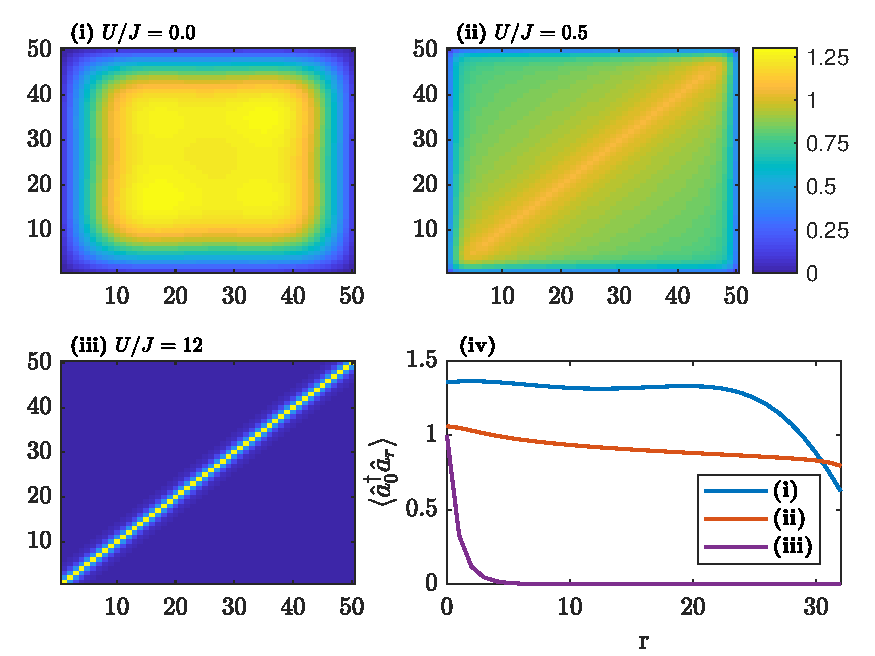
\includegraphics[width=\textwidth]{Figures/DensityMatrices.pdf}
    \caption{\textit{Density matrix of a 50 site system for various fractions of $U/J$. In \textbf{iv} the matrix entries of the 15th row is plotted as a function of distance from the diagonal, $r$. }}
    \label{fig:DensityMatrices}
\end{figure}
The figure depict the density matrix, with entries $\rho_{i,j} = \bra{\psi} \hat{a}_{i}^{\dag} \hat{a}_{j} \ket{\psi}$, of a system of size $N = 50$ with unit occupancy. The ground state $\ket{\psi}$ was found using the DMRG algorithm detailed in Section \ref{sec:DMRG}.
Figures \ref{fig:DensityMatrices}.i and \ref{fig:DensityMatrices}.iii show the density matrix plotted for the Superfluid and the Mott-Insulator limit respectively. In the Superfluid limit, long-range correlations are present, which is seen by large off-diagonal elements. However, since all correlations decay exponentially in the MPS description, the algorithm has difficulty approximating the very long range correlations of the system. This is visualized in figure \ref{fig:DensityMatrices}.iv, where the correlation function is plotted against distance from the diagonal. The Superfluid graph has a hump on it, which is an artifact of the DMRG algorithm. Due to the very long correlation length, the graph should be almost flat except for the rapid drop in the end, which is due to the open boundary conditions.\\
In the Mott-Insulator limit no interaction takes place between sites, and the correlation length is zero. Hence, the correlation matrix contains only diagonal elements of equal magnitude. Figure \ref{fig:DensityMatrices}.iii shows some off-diagonal elements of non-zero magnitude, however, this system is not a pure Mott-Insulator, as $U/J = 12$. Nevertheless, the correlations are well described by only a single exponential function, as seen by the figure.\\
Finally, figure \ref{fig:DensityMatrices}.ii illustrates the density matrix for a system with $U/J = 0.5$, which is primarily as Superfluid. The particles are not completely de-localized, which is noticeable from the well defined diagonal. Plotting the correlation function reveals the best approximation being a power-law, thus confirming the system is indeed a Superfluid. 



